\documentclass[12pt]{report}
\usepackage[a4paper, total={6in, 8in}]{geometry}
\usepackage{xcolor}
\usepackage{amsmath}
\usepackage{algpseudocode}
\usepackage{xcolor}
\usepackage{framed}
\usepackage{listings}
\lstset{basicstyle=\ttfamily,
  commentstyle=\color{red},
  keywordstyle=\color{blue},
  %basicstyle=\footnotesize,
  frame=lines,
  numbers=left,
  stepnumber=1,
  showstringspaces=false,
  tabsize=1,
  breaklines=true,
  breakatwhitespace=false,
}
\usepackage{hyperref}
\hypersetup
{
    colorlinks=true,
    linkcolor=blue,
    filecolor=magenta,
    urlcolor=cyan,
    pdftitle={\Huge \textbf{Software Systems Lab: OutLab}},
    pdfpagemode=FullScreen,
}
\usepackage[utf8]{inputenc}
\usepackage{graphicx}
\usepackage{longtable}
\usepackage{multirow}


\title{\Huge \textbf{Software Systems Lab: OutLab} \\ \textbf{\LaTeX{}}}
\author{\Large Name: Ashwin Abraham \\ \Large Roll no: 210050023}
\date{\Large September 6, 2022}

\begin{document}
\begin{titlepage}
    \maketitle
\end{titlepage}

\tableofcontents
\newpage

\chapter{Abstract}
\section{About this report}
This report was made by me as a part of my CS 251 course (Software Systems Lab).
This particular document was made as a part of the Outlab for the module on \LaTeX{}.
\section{Introduction}
In this report, I was supposed to make a report in \LaTeX{} showcasing my learning from previous labs in this report.
The following features were mandatory in this Outlab:
\begin{enumerate}
    \item \underline{\textbf{Frontpage}}
    \item \underline{\textbf{Table of Contents}}
    \item \underline{\textbf{Sections and Subsections}}
    \item \underline{\textbf{Table of Contents}}
    \item \underline{\textbf{Sections and Subsections}}
    \item \underline{\textbf{Use of Itemization}}
    \item \underline{\textbf{Images with Captions}}
    \item \underline{\textbf{A Table with Captions}}
    \item \underline{\textbf{Algorithm and Code}}
    \item \underline{\textbf{A minipage}}
    \item \underline{\textbf{A Bibliography}}
\end{enumerate}
The following points were also to be noted:
\begin{itemize}
    \item The report should be of \textbf{at least 5 pages} (10 points), including the front page and table of contents.
    \item You can use the article or report document class, and font size: 10-12pt.
    \item You can use the \underline{Overleaf} tool (An online \LaTeX{} editor).
    \item You can use online resources but don't forget to mention it in the readme and bibliography.
    \item Use \textbf{bold}, \textit{italic} and \underline{underlined} words wherever needed. \\ Also use new lines/paragraphs, proper spacing, etc..\\ You've to be creative with your work.
\end{itemize}
\section{Background in \LaTeX{}}
\subsection{Work done before this Module}
In the \textbf{PH 107} (\textit{Quantum Physics and Applications}) and \textbf{CH 107} (\textit{Quantum Chemistry}) courses, I used \LaTeX{} in order to submit
assignments. These assignments can be found in \href{https://github.com/AshwinAbraham2021}{my GitHub}: \href{https://github.com/AshwinAbraham2021/PH107-Resources}{here (PH 107)}, and
\href{https://github.com/AshwinAbraham2021/CH107-Resources}{here (CH 107)} \cite{github}. \LaTeX{} was aso used by me to prepare my \textit{Summer of Science} plan of action, mid-term and end-term reports on \textbf{Machine Learning},
which can be found \href{https://github.com/AshwinAbraham2021/SOS-Machine-Learning}{here}. It was also used for the \textbf{CS 215} (\textit{Data Analysis and Interpretation}) course assignments.
\subsection{Work done in this module}
As a part of the inlab for this module, we were asked to make a presentation using the \textit{Beamer} package
of \LaTeX{}, which is used for making slideshows and presentations. Then in the outlab, we were asked to make this report.


\chapter{Use of Itemization\cite{wikisort}}
\section{Itemization in Ordered Lists}
\begin{enumerate}
    \item Comparison based sorting algorithms\\
          These algorithms will always have $\Omega(n\log n)$ comparisons.
          \begin{enumerate}
              \item Sorting algorithms that are $O(n^2)$ on average
                    \begin{enumerate}
                        \item Bubble Sort
                        \item Insertion Sort
                        \item Selection Sort
                        \item Comb Sort
                        \item Exchange Sort
                        \item Shell Sort
                    \end{enumerate}
              \item Sorting algorithms that are $O(n\log n)$ on average
                    \begin{enumerate}
                        \item Merge Sort
                        \item Heap Sort
                        \item Quick Sort
                    \end{enumerate}
          \end{enumerate}
    \item Distribution based sorting algorithms\\
          These algorithms can be more efficient than $n\log n$ and are all $\Omega(n)$.\\
          However they make some assumptions about the distribution of the elements of the array.
          \begin{enumerate}
              \item Counting Sort\\
                    Here it is assumed that the elements of the array belong to a set $S$ of possibilities.\\
                    It's time complexity is then $O(n + |S|)$.
              \item Bucket Sort\\
                    Here we divide the array into $k$ buckets, and sort the buckets, and then merge them.\\
                    It's time complexity is $O(n + \frac{n^{2}}{k} + k)$.
              \item Radix Sort\\
                    Here we assume that the elements are to be sorted lexicographically.\\
                    It's time complexity is $O(wn)$ where $w$ is the length of each element.
          \end{enumerate}
\end{enumerate}

\section{Itemization in Unordered Lists}
The same thing, but as an unordered list.
\begin{itemize}
    \item Comparison based sorting algorithms\\
          These algorithms will always have $\Omega(n\log n)$ comparisons.
          \begin{itemize}
              \item Sorting algorithms that are $O(n^2)$ on average
                    \begin{itemize}
                        \item Bubble Sort
                        \item Insertion Sort
                        \item Selection Sort
                        \item Comb Sort
                        \item Exchange Sort
                        \item Shell Sort
                    \end{itemize}
              \item Sorting algorithms that are $O(n\log n)$ on average
                    \begin{itemize}
                        \item Merge Sort
                        \item Heap Sort
                        \item Quick Sort
                    \end{itemize}
          \end{itemize}
    \item Distribution based sorting algorithms\\
          These algorithms can be more efficient than $n\log n$ and are all $\Omega(n)$.\\
          However they make some assumptions about the distribution of the elements of the array.
          \begin{itemize}
              \item Counting Sort\\
                    Here it is assumed that the elements of the array belong to a set $S$ of possibilities.\\
                    It's time complexity is then $O(n + |S|)$.
              \item Bucket Sort\\
                    Here we divide the array into $k$ buckets, and sort the buckets, and then merge them.\\
                    It's time complexity is $O(n + \frac{n^{2}}{k} + k)$.
              \item Radix Sort\\
                    Here we assume that the elements are to be sorted lexicographically.\\
                    It's time complexity is $O(wn)$ where $w$ is the length of each element.
          \end{itemize}
\end{itemize}


\chapter{Images with Captions}
Have a look at these images with captions related to sorting.
\begin{figure}[h!]
    \centering
    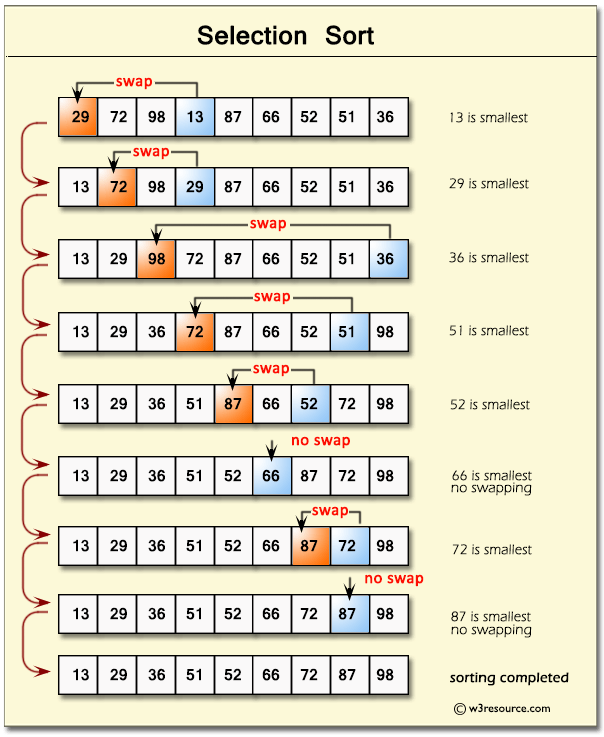
\includegraphics[width=0.6\textwidth]{images/selection-sort.png}
    \caption{Selection Sort\cite{ssort}}
\end{figure}
\begin{figure}[h!]
    \centering
    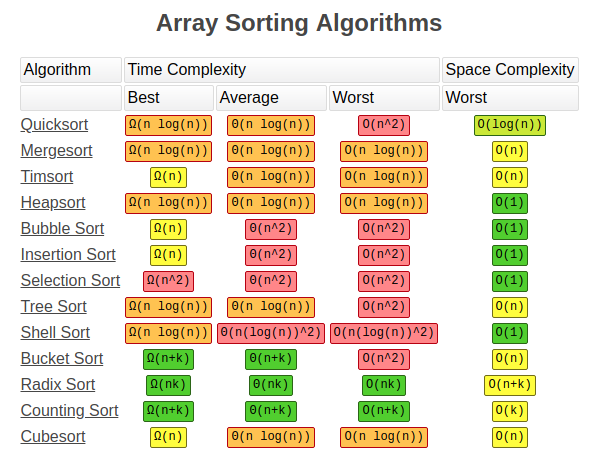
\includegraphics[width=0.8\textwidth]{images/complexities.png}
    \caption{Time Complexities of some Sorting Algorithms\cite{complexities}}
\end{figure}

\chapter{A Table with Captions}

\begin{table}[h!]
    \begin{tabular}{ |p{2.5cm}||p{2.5cm}|p{2.5cm}|p{2.5cm}|p{2.5cm}|  }
        \hline
        \multicolumn{5}{|c|}{Sorting Algorithms} \\
        \hline
        \centering Algorithm& \centering Best Case Complexity & \centering Average Case Complexity&\centering Worst Case Complexity& Memory Complexity\\
        \hline
        \centering Bubblesort & \centering $\Omega(n)$ & \centering $\Theta(n^{2})$ & \centering $O(n^{2})$ & $O(1)$\\
        \hline
        \centering Insertion Sort & \centering $\Omega(n)$ & \centering $\Theta(n^{2})$ & \centering $O(n^{2})$ & $O(1)$\\
        \hline
        \centering Selection Sort & \centering $\Omega(n^{2})$ & \centering $\Theta(n^{2})$ & \centering $O(n^{2})$ & $O(1)$\\
        \hline
        \centering Comb Sort & \centering $\Omega(n\log n)$ & \centering $\Theta(n^{2})$ & \centering $O(n^{2})$ & $O(1)$\\
        \hline
        \centering Exchange Sort & \centering $\Omega(n^{2})$ & \centering $\Theta(n^{2})$ & \centering $O(n^{2})$ & $O(1)$\\
        \hline
        \centering Shell Sort & \centering $\Omega(n\log n)$ & \centering $\Theta(n^{\frac{4}{3}})$ & \centering $O(n^{\frac{3}{2}})$ & $O(1)$\\
        \hline
        \centering Merge Sort & \centering $\Omega(n\log n)$ & \centering $\Theta(n\log n)$ & \centering $O(n\log n)$ & $O(n)$\\
        \hline
        \centering Heap Sort & \centering $\Omega(n\log n)$ & \centering $\Theta(n\log n)$ & \centering $O(n\log n)$ & $O(1)$\\
        \hline
        \centering Quick Sort & \centering $\Omega(n\log n)$ & \centering $\Theta(n\log n)$ & \centering $O(n^{2})$ & $O(\log n)$\\
        \hline
        \centering Counting Sort & \centering $\Omega(n + r)$ & \centering $\Theta(n + r)$ & \centering $O(n + r)$ & $O(n + r)$\\
        \hline
        \centering Bucket Sort & \centering $\Omega(n + r)$ & \centering $\Theta(n + r)$ & \centering $O(n + r)$ & $O(n + r)$\\
        \hline
        \centering Radix Sort & \centering $\Omega(n)$ & \centering $\Theta(n\frac{k}{d})$ & \centering $O(n\frac{k}{d})$ & $O(n + 2^{d})$\\
        \hline
    \end{tabular}
    \caption{Some popular sorting algorithms and their complexities\cite{wikisort}}
\end{table}

\chapter{Algorithm and Code}
Here we will discuss an algorithm to print the first $n$ Fibonacci numbers.
This was part of the second inlab of \textbf{CS 251}.
The pseudocode of this algorithm is as follows:
\begin{algorithmic}[1]
    \State $x \gets 0$
    \State $y \gets 1$
    \For{$k \gets 1$ to $n$}
    \State \textbf{print} $x$
    \State $temp \gets x$
    \State $x \gets y$
    \State $y \gets y + temp$
    \EndFor
\end{algorithmic}
The implementation of this algorithm as a \textit{Bash} Script \cite{cs251} is as follows:

\begin{lstlisting}[language=bash,caption={Calculating the Fibonacci Numbers}]
#! /bin/bash

x=0
y=1
str=""
num=$(($1))
for ((i=0; i<$num; i++))
do
    str+="$x "
    temp=$(($x))
    x=$(($y))
    y=$(($y+$temp))
done
echo $str
\end{lstlisting}

\chapter{Minipage}
The following is a boxed minipage.\\
\fbox{
    \begin{minipage}{6cm}
        Lorem ipsum\cite{loremipsum} dolor sit amet, consectetur adipiscing elit,
        sed do eiusmod tempor incididunt ut labore et dolore magna aliqua.\\ 
        Ut enim ad minim veniam, quis nostrud exercitation ullamco laboris nisi ut aliquip ex ea commodo consequat.\\
        Duis aute irure dolor in reprehenderit in voluptate velit esse cillum dolore eu fugiat nulla pariatur.\\
        Excepteur sint occaecat cupidatat non proident, sunt in culpa qui officia deserunt mollit anim id est laborum.
    \end{minipage}
}
\bibliographystyle{plain}
\bibliography{refs}
\end{document}